\documentclass[10pt,a4paper]{article}

\usepackage[top=18mm,bottom=16mm,left=16mm,right=16mm]{geometry}
\usepackage[T1]{fontenc}
\usepackage{tgheros}
\renewcommand{\familydefault}{\sfdefault}
\usepackage{microtype}
\usepackage{amsmath}

\usepackage[dvipsnames,svgnames,x11names]{xcolor}
\definecolor{bg}{HTML}{0E0E11}
\definecolor{cardbg}{HTML}{1F2937}
\definecolor{cyan}{HTML}{00D4FF}
\definecolor{gold}{HTML}{D4A574}
\definecolor{brightgold}{HTML}{FFD700}
\definecolor{crimson}{HTML}{E94560}
\definecolor{purple}{HTML}{8B5CF6}
\definecolor{emerald}{HTML}{10B981}
\definecolor{amber}{HTML}{F59E0B}
\definecolor{textmain}{HTML}{F0EDED}
\definecolor{textmuted}{HTML}{9CA3AF}
\definecolor{accentbar}{HTML}{00D4FF}

\usepackage{graphicx}
\graphicspath{{img/}}
\usepackage{tikz}
\usetikzlibrary{calc,positioning,backgrounds,fit,arrows.meta}
\usepackage{multicol}
\usepackage{enumitem}
\usepackage{tabularx}
\usepackage{booktabs}
\usepackage{fontawesome5}
\usepackage{hyperref}
\hypersetup{colorlinks=true,urlcolor=cyan,linkcolor=cyan,citecolor=gold}
\usepackage{ragged2e}
\usepackage{setspace}
\usepackage{fancyhdr}
\usepackage{lastpage}
\usepackage{colortbl}

\pagecolor{bg}
\color{textmain}

\fancypagestyle{branded}{%
  \fancyhf{}
  \renewcommand{\headrulewidth}{0pt}
  \renewcommand{\footrulewidth}{0.4pt}
  \renewcommand{\footrule}{\hbox to\headwidth{\color{cyan}\leaders\hrule height \footrulewidth\hfill}}
  \fancyfoot[L]{\tiny\color{textmuted}VisionFlow Ecosystem Pitch | DreamLab AI}
  \fancyfoot[R]{\tiny\color{textmuted}\thepage\,/\,\pageref{LastPage}}
}
\pagestyle{branded}

\setlength{\parindent}{0pt}
\setlength{\parskip}{4pt}
\setlength{\columnsep}{8mm}

\newcommand{\sectiontag}[1]{%
  \vspace{6pt}%
  {\footnotesize\color{gold}\MakeUppercase{#1}}\\[-1pt]%
}
\newcommand{\accentrule}{\textcolor{cyan}{\rule{\linewidth}{0.5pt}}}
\newcommand{\stat}[2]{%
  {\Large\bfseries\color{cyan}#1}\\[-2pt]%
  {\tiny\color{textmuted}#2}%
}

\begin{document}

% ═══════════════════════════════════════════════
% COVER / TITLE
% ═══════════════════════════════════════════════
\begin{tikzpicture}[remember picture, overlay]
  \fill[accentbar] (current page.north west) rectangle ([yshift=-3pt]current page.north east);
\end{tikzpicture}

\vspace{-2mm}

\begin{center}
  {\color{cyan}\Huge$\diamondsuit$}\\[4pt]
  {\Huge\bfseries VisionFlow}\\[2pt]
  {\Large\color{gold}Coordination Engineering for Federated Human--AI Intelligence}\\[6pt]
  {\small\color{textmuted}Ecosystem Technical Pitch \quad|\quad May 2026}\\[2pt]
  {\small\color{textmuted}Dr John O'Hare \quad|\quad DreamLab AI \quad|\quad \href{https://www.visionflow.info}{visionflow.info}}
\end{center}

\vspace{4pt}
\accentrule
\vspace{2pt}

\begin{center}
\begin{tabular}{c@{\hspace{14mm}}c@{\hspace{14mm}}c@{\hspace{14mm}}c@{\hspace{14mm}}c@{\hspace{14mm}}c}
  \stat{5}{Federated Substrates} &
  \stat{92}{CUDA Kernels} &
  \stat{185+}{MCP Tools} &
  \stat{55\texttimes}{GPU Speedup} &
  \stat{120K+}{Lines of Rust} &
  \stat{6}{OSS Repos}
\end{tabular}
\end{center}

\vspace{2pt}
\accentrule

% ═══════════════════════════════════════════════
% EXECUTIVE SUMMARY
% ═══════════════════════════════════════════════
\vspace{4pt}

\sectiontag{Executive Summary}

{\small
VisionFlow is an open-source coordination harness for federated human--AI intelligence. It solves the governance gap that emerges when organisations deploy multiple AI agents. Without shared semantics, cryptographic identity, and human-in-the-loop oversight, agents waste 60--80\% of tokens on context rediscovery, duplicate reasoning, and contradictory outputs.

Six federated repositories. 120K+ lines of Rust. 92 CUDA kernels. 185+ MCP tools. Five independent substrates mesh through a single cryptographic identity spine (\texttt{did:nostr} secp256k1). Every actor (human, agent, server) authenticates at every layer via the same keypair, enabling federation without centralised infrastructure.

\textbf{For token and model vendors:} VisionFlow is the coordination layer that makes extreme token consumption against hard problems rational. Shared ontology eliminates re-derivation. Provenance chains eliminate re-validation. Judgment Broker eliminates decision spin. Result: 3--5\texttimes{} effective token throughput gain, with every token producing auditable, governed, provenance-tracked reasoning.
}

% ═══════════════════════════════════════════════
% THE PROBLEM
% ═══════════════════════════════════════════════
\sectiontag{Coordination Failure at Scale}

\begin{multicols}{2}
\raggedright

{\small
AI has moved through a clear progression: LLM $\to$ chatbot $\to$ reasoning $\to$ agent $\to$ agentics $\to$ external harness. Each stage solves the previous stage's limitation and reveals a new one. VisionFlow occupies the next position: the \textbf{coordination harness}, providing shared semantics, federated identity, governance, and cryptographic provenance.

\textbf{73\% of frontline AI adoption happens without management sign-off.} Your workforce is already building shadow workflows, stitching together AI agents, automating procurement shortcuts. Your organisation is becoming an agentic mesh whether you plan for it or not.
}

\columnbreak

{\small
\textbf{Four failure modes of uncoordinated AI:}
\begin{itemize}[leftmargin=8pt,itemsep=1pt,parsep=0pt,topsep=2pt,label={\color{crimson}\faTimes}]
  \item \textbf{Centralised AI} scales tokens but not trust. One vendor, one failure mode, one billing relationship.
  \item \textbf{Agent frameworks} scale tasks but not governance. Fast and broken is still broken.
  \item \textbf{Knowledge tools} scale information but not reasoning. More data doesn't mean better decisions.
  \item \textbf{Collaboration platforms} scale communication but not coordination. More Slack channels don't solve alignment.
\end{itemize}
}

\end{multicols}

% ═══════════════════════════════════════════════
% ECOSYSTEM ARCHITECTURE
% ═══════════════════════════════════════════════
\sectiontag{Ecosystem Architecture: Five Substrates, One Identity}

\begin{center}
  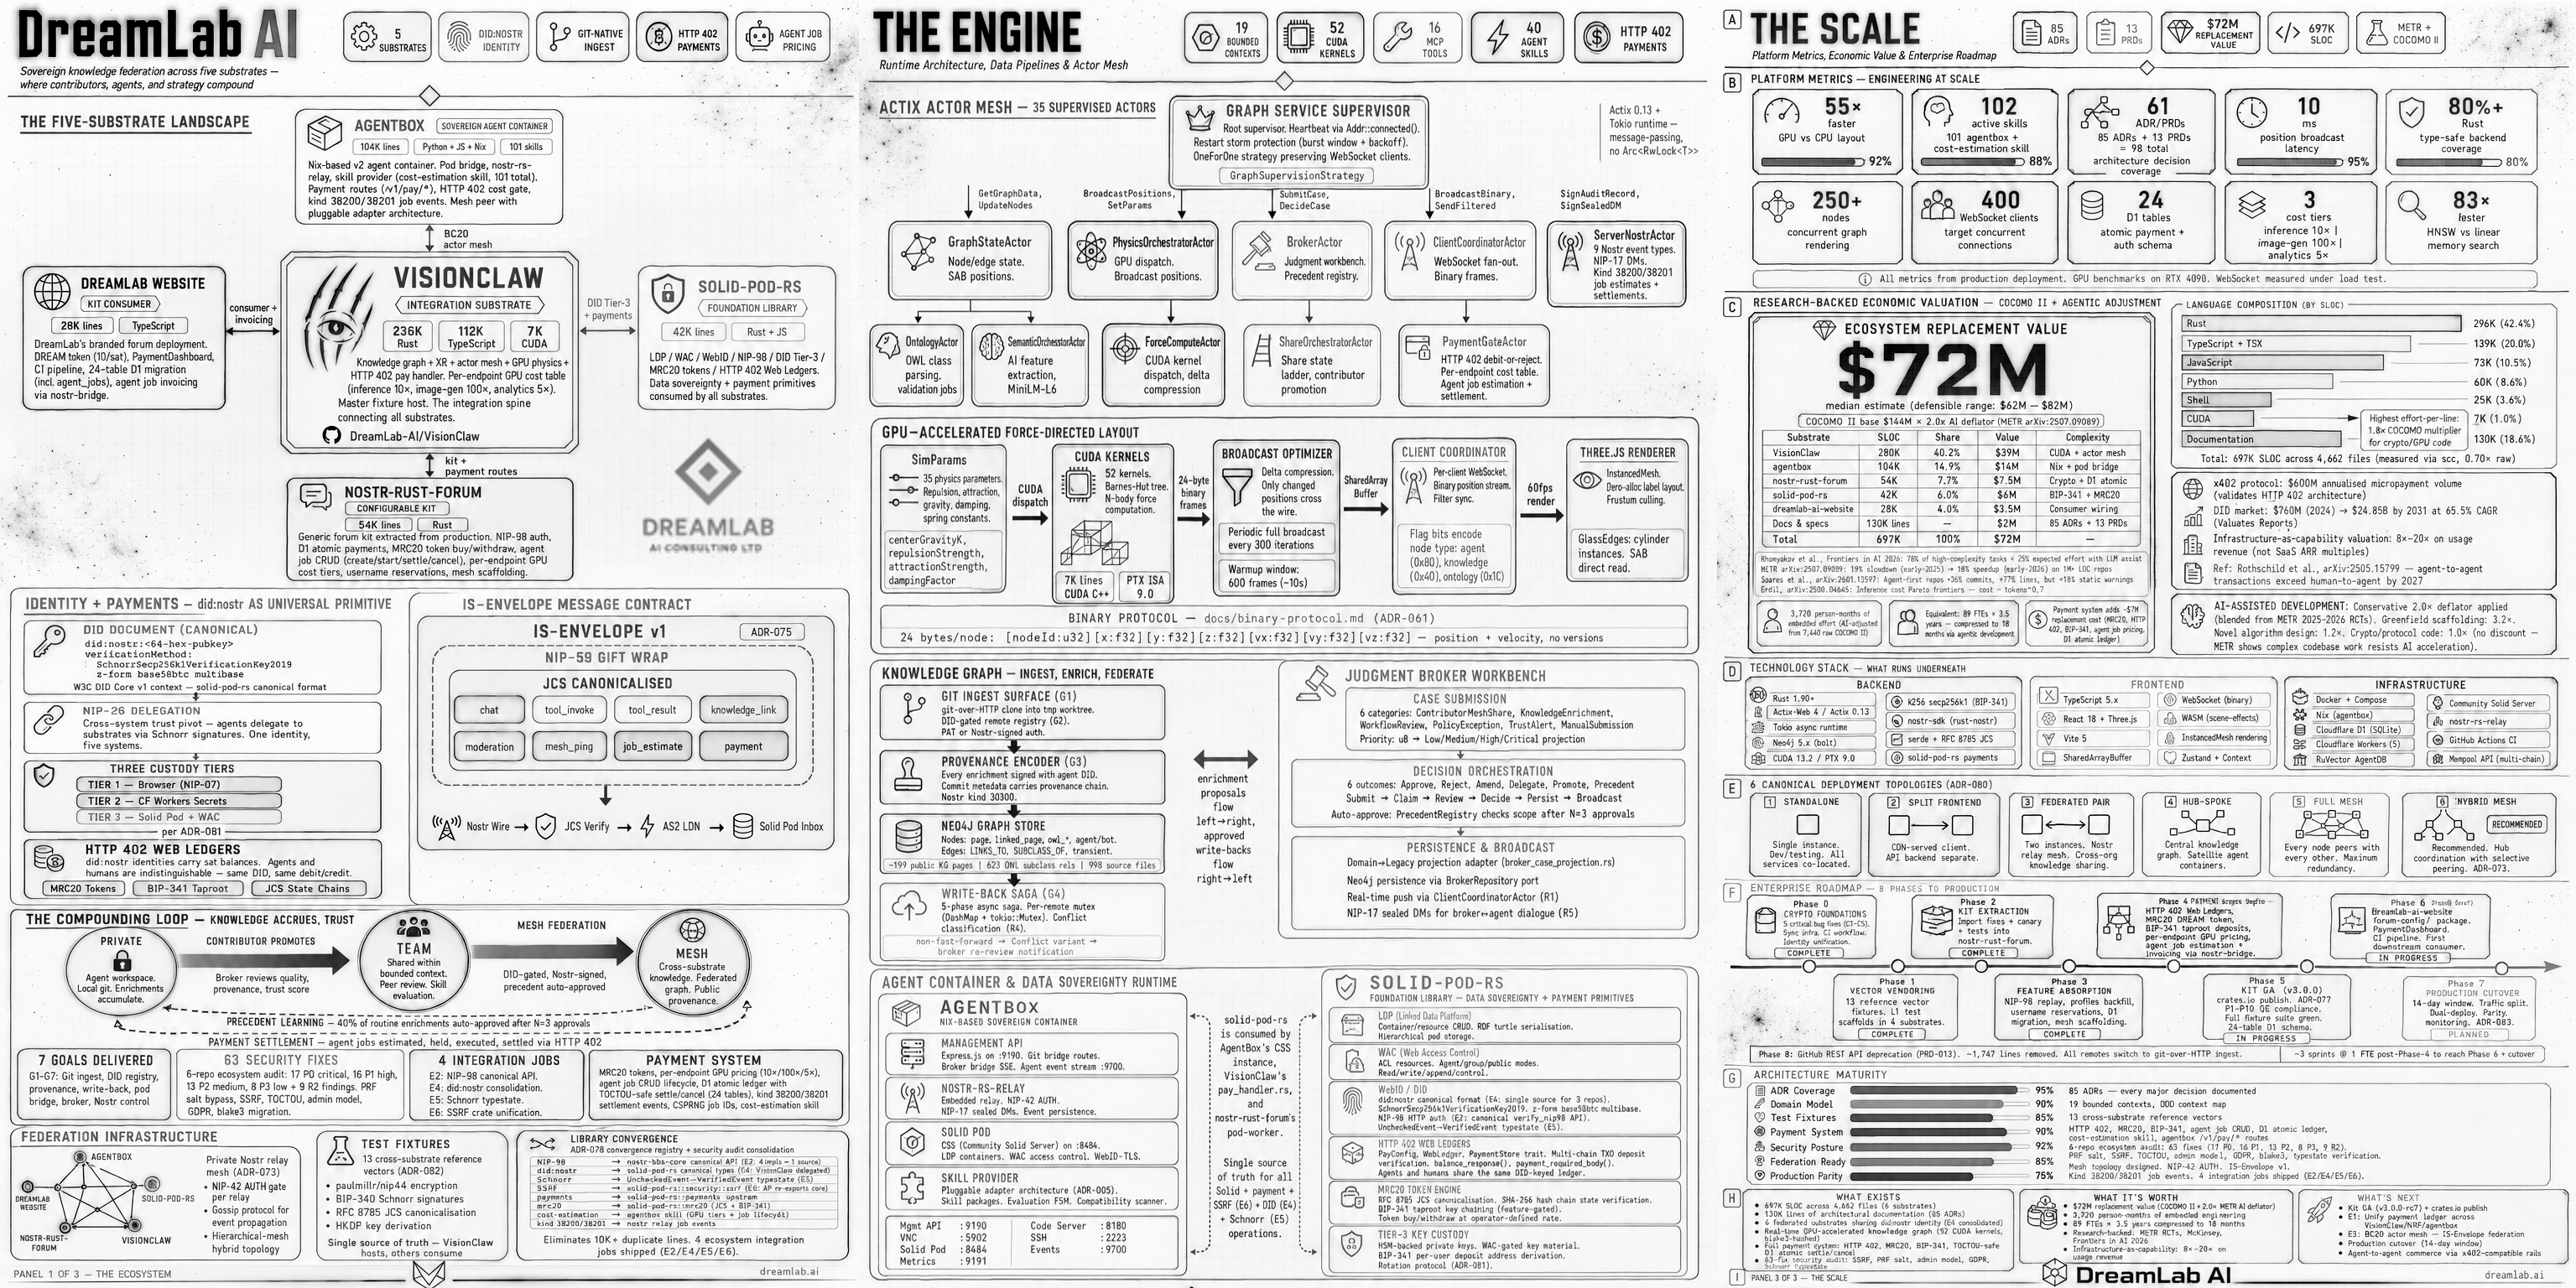
\includegraphics[width=0.85\linewidth]{../assets/diagrams/ecosystem-overview.png}
\end{center}

\vspace{2pt}

{\small Every actor (human, agent, server, worker) shares a single \texttt{did:nostr:<hex-pubkey>} secp256k1 keypair. Verified at the Nostr relay, at every HTTP request (NIP-98 Schnorr), against WAC ACLs on Solid pods, in every provenance bead, and resolvable as a W3C DID Document.}

\vspace{4pt}

\begin{multicols}{2}
\raggedright

% ── SUBSTRATE 1: VisionClaw ──
{\color{cyan}\faProjectDiagram}\;\;{\normalsize\bfseries\color{cyan}VisionClaw | Knowledge Engineering}\\[2pt]
{\small
\begin{itemize}[leftmargin=8pt,itemsep=0pt,parsep=0pt,topsep=1pt,label={\color{cyan}\textbullet}]
  \item OWL 2 EL formal reasoning via Whelk-rs: provably correct entailments from description logic, not statistical inference
  \item 92 CUDA kernels: semantic relationships become GPU physics forces (\texttt{subClassOf} $\to$ attraction, \texttt{disjointWith} $\to$ repulsion). 55\texttimes{} speedup vs CPU
  \item 934-node force-directed 3D graph with real-time rendering
  \item 17 MCP ontology tools (7 native + 10 bridge to SPARQL)
  \item Immersive XR built on 15 years of CAVE research at University of Salford. Migrating to native Quest 3 APK (Godot 4 + godot-rust + OpenXR)
  \item THG world record: 250+ concurrent VR users in knowledge graph
  \item 10 DDD bounded contexts, 114 command/query handlers, CQRS architecture
\end{itemize}
\textbf{Maturity:} $\sim$120K LOC Rust. Production. GPU physics, graph rendering, ontology tools all operational. XR layer experimental.\\
\textbf{Licence:} MPL 2.0. Commercial use permitted. Modifications to MPL files must be shared.
}

\vspace{6pt}

% ── SUBSTRATE 2: Agentbox ──
{\color{purple}\faCogs}\;\;{\normalsize\bfseries\color{purple}Agentbox | Harness Engineering}\\[2pt]
{\small
\begin{itemize}[leftmargin=8pt,itemsep=0pt,parsep=0pt,topsep=1pt,label={\color{purple}\textbullet}]
  \item Hardened Nix-built container, byte-for-byte reproducible. Non-root, read-only filesystem, capabilities dropped
  \item 90+ agent skills, 185+ MCP tools (Playwright, ComfyUI, QGIS, Blender, LaTeX, Jupyter, PyTorch)
  \item Multi-runtime: Claude Code, Codex, Gemini, DeepSeek, Ruflo
  \item 5-slot pluggable adapter architecture: beads, pods, memory, events, orchestrator
  \item Embedded Solid Pod server (solid-pod-rs) + Nostr relay (nostr-rs-relay)
  \item BIP-340 sovereign identity at bootstrap. Agents own their keys
  \item Privacy filter sidecar for PII redaction before any log or telemetry
  \item Browser-based setup wizard, zero external dependencies
  \item 18 URN kinds for resource naming (\texttt{urn:agentbox:<kind>:[<scope>:]<local>})
\end{itemize}
\textbf{Maturity:} Production core. 620+ line manifest. 20+ architecture docs (ADRs/PRDs/DDDs). Security audit hardened May 2026.\\
\textbf{Licence:} AGPL 3.0. Network-service copyleft (upstream JSS). Commercial licensing available via Melvin Carvalho.
}

\columnbreak

% ── SUBSTRATE 3: solid-pod-rs ──
{\color{emerald}\faLock}\;\;{\normalsize\bfseries\color{emerald}solid-pod-rs | Cryptographic Foundation}\\[2pt]
{\small
\begin{itemize}[leftmargin=8pt,itemsep=0pt,parsep=0pt,topsep=1pt,label={\color{emerald}\textbullet}]
  \item Rust port of JavaScriptSolidServer (JSS), 98\% parity. 201 rows tracked: 158 present, 5 partial, 3 missing
  \item W3C Solid Protocol: LDP, WAC access control, conditional requests, glob GET
  \item Dual auth: NIP-98 Schnorr (stateless) + Solid-OIDC with DPoP (RFC 9449)
  \item Full identity provider crate: OIDC authorization-code flow, dynamic client registration, WebAuthn passkeys, NIP-07 Schnorr SSO
  \item HTTP 402 micropayments: WAC PaymentCondition, per-read satoshi costs, MRC20 token minting, BIP-341 anchoring
  \item ActivityPub federation: inbox/outbox, HTTP Signature verification, follower fan-out
  \item Git HTTP backend: smart protocol, NIP-98 bridge auth, WAC-integrated
  \item Embedded NIP-01 Nostr relay with DID Document publication
  \item Dual compile: native Tokio + WASM Cloudflare Workers
  \item 870+ tests, SSRF hardened, dotfile allowlist, path traversal protection
\end{itemize}
\textbf{Maturity:} v0.4.0-alpha.15. $\sim$20K LOC across 6 crates. Feature-complete, pre-1.0 stabilisation.\\
\textbf{Licence:} AGPL 3.0. Network-service copyleft (upstream JSS). Commercial licensing available via Melvin Carvalho.
}

\vspace{6pt}

% ── SUBSTRATE 4: nostr-rust-forum ──
{\color{gold}\faBalanceScale}\;\;{\normalsize\bfseries\color{gold}nostr-rust-forum | Governance UI \& Relay Kit}\\[2pt]
{\small
\begin{itemize}[leftmargin=8pt,itemsep=0pt,parsep=0pt,topsep=1pt,label={\color{gold}\textbullet}]
  \item 12 Rust crates: core protocol, 5 Cloudflare Workers, Leptos WASM client, mesh federation, rate limiting, config, search, setup
  \item Judgment Broker decision surface: 1,015-line governance model
  \item Agent Control Surface Protocol: kinds 31400--31405 (PanelDefinition, PanelState, ActionRequest, ActionResponse, PanelUpdate, PanelRetired)
  \item REST governance API: 7 NIP-98-gated endpoints (agent registry, broker cases/decisions, roles)
  \item Passkey-first auth: WebAuthn PRF derives Nostr keys deterministically. No passwords stored
  \item 3-zone access: public, members, private (runtime configurable)
  \item Leptos WASM client: 19 pages, 60+ components, governance dashboard, admin panel
  \item 15 NIP implementations (NIP-01/07/09/29/33/40/42/44/45/50/52/98 + custom 31400--31405)
  \item Two-tier pod storage: CF Workers (auto-provisioned) + native solid-pod-rs (git-capable)
  \item Vector search (NIP-50): in-memory cosine k-NN, RVF binary format
\end{itemize}
\textbf{Maturity:} v3.0.0-rc7. Phase 1 sprint complete (federated NIP-05, pod-resident keys, data export). Actively deployed.\\
\textbf{Licence:} Dual MIT / Apache-2.0. Permissive. No copyleft obligation on the forum crate itself.
}

\end{multicols}

% ── SUBSTRATE 5: DreamLab Edge ──
\vspace{2pt}
{\color{crimson}\faGlobe}\;\;{\normalsize\bfseries\color{crimson}DreamLab Edge | Branded Deployment} {\small\color{textmuted}| React SPA + Leptos WASM forum on Cloudflare Workers | Operator overlay configuration | Live at \href{https://dreamlab-ai.com}{dreamlab-ai.com} | Consumes all substrates as library crates}

% ═══════════════════════════════════════════════
% JUDGMENT BROKER
% ═══════════════════════════════════════════════
\newpage

\sectiontag{Judgment Broker: Human-in-the-Loop Governance}

{\small Judgment Broker is an emergent property of agents, humans, a knowledge graph, and a relay mesh coordinating through shared cryptographic identity. No single repository owns it.}

\vspace{4pt}

\begin{center}
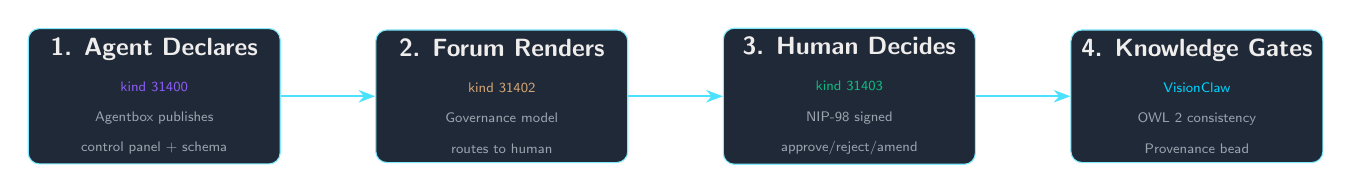
\begin{tikzpicture}[
  node distance=0.8cm and 1.2cm,
  bstep/.style={draw=cyan!50,fill=cardbg,rounded corners=4pt,
               text=textmain,font=\small,align=center,
               minimum width=3.2cm,minimum height=1.6cm},
  arr/.style={-{Stealth[length=6pt]},cyan!70,thick}
]
  \node[bstep] (s1) {\textbf{1. Agent Declares}\\[2pt]{\tiny\color{purple}kind 31400}\\{\tiny\color{textmuted}Agentbox publishes}\\{\tiny\color{textmuted}control panel + schema}};
  \node[bstep,right=of s1] (s2) {\textbf{2. Forum Renders}\\[2pt]{\tiny\color{gold}kind 31402}\\{\tiny\color{textmuted}Governance model}\\{\tiny\color{textmuted}routes to human}};
  \node[bstep,right=of s2] (s3) {\textbf{3. Human Decides}\\[2pt]{\tiny\color{emerald}kind 31403}\\{\tiny\color{textmuted}NIP-98 signed}\\{\tiny\color{textmuted}approve/reject/amend}};
  \node[bstep,right=of s3] (s4) {\textbf{4. Knowledge Gates}\\[2pt]{\tiny\color{cyan}VisionClaw}\\{\tiny\color{textmuted}OWL 2 consistency}\\{\tiny\color{textmuted}Provenance bead}};
  \draw[arr] (s1) -- (s2);
  \draw[arr] (s2) -- (s3);
  \draw[arr] (s3) -- (s4);
\end{tikzpicture}
\end{center}

\vspace{4pt}

{\small
\begin{tabularx}{\linewidth}{@{}lllX@{}}
  \toprule
  \textbf{\color{textmuted}Kind} & \textbf{\color{textmuted}Name} & \textbf{\color{textmuted}Direction} & \textbf{\color{textmuted}Purpose} \\
  \midrule
  \texttt{31400} & PanelDefinition & Agent $\to$ Relay & Declare control panel with schema, fields, and actions \\
  \texttt{31401} & PanelState & Agent $\to$ Relay & Current data snapshot \\
  \texttt{31402} & ActionRequest & Agent $\to$ Relay & Request human decision \\
  \texttt{31403} & ActionResponse & Human $\to$ Relay & Cryptographically signed approve/reject/amend/delegate \\
  \texttt{31404} & PanelUpdate & Agent $\to$ Relay & Incremental state diff \\
  \texttt{31405} & PanelRetired & Agent $\to$ Relay & Retire panel \\
  \bottomrule
\end{tabularx}
}

\vspace{2pt}
{\small Every decision is an immutable Nostr event. In regulated industries (pharma, finance, defence), reconstructing decision provenance after the fact costs orders of magnitude more than generating it by construction. Result: \textbf{90\% reduction in audit reconstruction cost}.}

% ═══════════════════════════════════════════════
% TOKEN ECONOMICS
% ═══════════════════════════════════════════════
\sectiontag{Token Economics: Why Tokenmaxing for Hard Problems Is Rational}

\begin{multicols}{2}
\raggedright

{\small
\textbf{Cost of not coordinating.} A 50-person team running uncoordinated AI agents wastes \textbf{5--8\texttimes{} tokens} on context rediscovery, duplicate reasoning, and contradictory outputs. Each agent session starts cold: no shared ontology, no provenance, no memory of what other agents concluded.

\textbf{Coordination as token multiplier.} Shared ontology means agents stop re-deriving domain vocabulary. Provenance chain means agents stop re-validating conclusions. Judgment Broker means agents stop spinning on decisions they lack authority to make. Result: \textbf{3--5\texttimes{} effective throughput gain}.

\textbf{Hard problems justify deep spend.}
\begin{itemize}[leftmargin=8pt,itemsep=1pt,parsep=0pt,topsep=2pt,label={\color{cyan}\textbullet}]
  \item Drug discovery: \$2.6B average cost per approved compound
  \item Climate modelling: \$50M+ per actionable simulation suite
  \item Creative production: \$100M+ per franchise
\end{itemize}
Against these stakes, \$10K--100K on coordinated AI reasoning is a rounding error, provided the coordination harness prevents even one wrong conclusion from propagating.
}

\columnbreak

\begin{center}
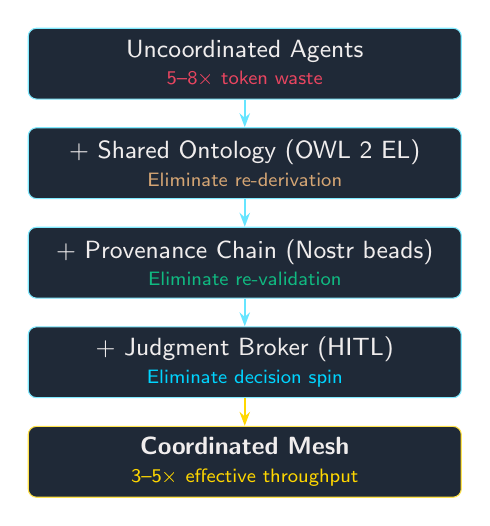
\begin{tikzpicture}[
  node distance=0.35cm,
  box/.style={draw=cyan!50,fill=cardbg,rounded corners=3pt,
              text=textmain,font=\small,align=center,
              minimum width=5.5cm,minimum height=0.9cm}
]
  \node[box] (a) {Uncoordinated Agents\\[-1pt]{\scriptsize\color{crimson}5--8\texttimes{} token waste}};
  \node[box,below=of a] (b) {+ Shared Ontology (OWL 2 EL)\\[-1pt]{\scriptsize\color{gold}Eliminate re-derivation}};
  \node[box,below=of b] (c) {+ Provenance Chain (Nostr beads)\\[-1pt]{\scriptsize\color{emerald}Eliminate re-validation}};
  \node[box,below=of c] (d) {+ Judgment Broker (HITL)\\[-1pt]{\scriptsize\color{cyan}Eliminate decision spin}};
  \node[box,below=of d,draw=brightgold!70] (e) {\bfseries Coordinated Mesh\\[-1pt]{\scriptsize\color{brightgold}3--5\texttimes{} effective throughput}};
  \draw[-{Stealth[length=5pt]},cyan!60,thick] (a) -- (b);
  \draw[-{Stealth[length=5pt]},cyan!60,thick] (b) -- (c);
  \draw[-{Stealth[length=5pt]},cyan!60,thick] (c) -- (d);
  \draw[-{Stealth[length=5pt]},brightgold,thick] (d) -- (e);
\end{tikzpicture}
\end{center}

\vspace{4pt}

{\small\textbf{ROI model:}}\\
{\small $\mathrm{ROI} = \dfrac{V \times \mathrm{coordination\_mult} \times \mathrm{governance\_div}}{\mathrm{token\_cost} \times N}$}

\vspace{4pt}
{\small Break-even at \textbf{3 agents} on any problem valued above \textbf{\$50K}. Beyond that, every additional coordinated agent produces net positive value. Ontology, identity spine, and governance plane are shared infrastructure.}

\end{multicols}

% ═══════════════════════════════════════════════
% COMPETITIVE LANDSCAPE
% ═══════════════════════════════════════════════
\sectiontag{Competitive Landscape}

{\small Every differentiator sits where no competitor can follow. All competing platforms cluster in the commodity zone.}

\vspace{4pt}

{\small\renewcommand{\arraystretch}{1.2}
\begin{tabularx}{\linewidth}{@{}X*{6}{c}@{}}
  \toprule
  \textbf{\color{textmuted}Platform} & \textbf{\color{textmuted}Crypto Identity} & \textbf{\color{textmuted}Data Sovereignty} & \textbf{\color{textmuted}Governance} & \textbf{\color{textmuted}Formal Reasoning} & \textbf{\color{textmuted}Federation} & \textbf{\color{textmuted}OSS} \\
  \midrule
  \rowcolor{cardbg}
  \textbf{VisionFlow} & {\color{emerald}\faCheck} & {\color{emerald}\faCheck} & {\color{emerald}\faCheck} & {\color{emerald}\faCheck} & {\color{emerald}\faCheck} & {\color{emerald}\faCheck} \\
  Google Spark & {\color{crimson}\faTimes} & {\color{crimson}\faTimes} & {\color{gold}$\sim$} & {\color{crimson}\faTimes} & {\color{crimson}\faTimes} & {\color{crimson}\faTimes} \\
  OpenAI Codex & {\color{crimson}\faTimes} & {\color{crimson}\faTimes} & {\color{crimson}\faTimes} & {\color{crimson}\faTimes} & {\color{crimson}\faTimes} & {\color{gold}$\sim$} \\
  Claude Code & {\color{crimson}\faTimes} & {\color{gold}$\sim$} & {\color{gold}$\sim$} & {\color{crimson}\faTimes} & {\color{gold}$\sim$} & {\color{gold}$\sim$} \\
  Devin & {\color{crimson}\faTimes} & {\color{crimson}\faTimes} & {\color{gold}$\sim$} & {\color{crimson}\faTimes} & {\color{crimson}\faTimes} & {\color{crimson}\faTimes} \\
  CrewAI & {\color{crimson}\faTimes} & {\color{gold}$\sim$} & {\color{gold}$\sim$} & {\color{crimson}\faTimes} & {\color{gold}$\sim$} & {\color{emerald}\faCheck} \\
  AutoGen & {\color{crimson}\faTimes} & {\color{gold}$\sim$} & {\color{gold}$\sim$} & {\color{crimson}\faTimes} & {\color{gold}$\sim$} & {\color{emerald}\faCheck} \\
  LangGraph & {\color{crimson}\faTimes} & {\color{gold}$\sim$} & {\color{gold}$\sim$} & {\color{crimson}\faTimes} & {\color{gold}$\sim$} & {\color{emerald}\faCheck} \\
  Cursor / Windsurf & {\color{crimson}\faTimes} & {\color{gold}$\sim$} & {\color{gold}$\sim$} & {\color{crimson}\faTimes} & {\color{crimson}\faTimes} & {\color{crimson}\faTimes} \\
  \bottomrule
\end{tabularx}}

\vspace{2pt}
{\scriptsize\color{textmuted}{\color{emerald}\faCheck}\,Protocol-native \quad {\color{gold}$\sim$}\,Partial/add-on \quad {\color{crimson}\faTimes}\,Absent}

\vspace{4pt}

\begin{multicols}{3}
\raggedright
{\small
\textbf{\color{emerald}Formal Reasoning: Solid Red}\\
Every competitor relies on probabilistic LLM inference. VisionFlow's OWL 2 EL subsumption produces provably correct entailments.

\columnbreak

\textbf{\color{emerald}Crypto Identity: Solid Red}\\
Only VisionFlow implements cryptographic agent identity at the protocol level. Every other platform ties identity to someone else's server.

\columnbreak

\textbf{\color{emerald}Federation: Solid Red}\\
No competitor supports sovereign nodes trusting each other via cryptographic identity rather than shared infrastructure.
}
\end{multicols}

% ═══════════════════════════════════════════════
% USE CASES
% ═══════════════════════════════════════════════
\sectiontag{Real-World Scenarios}

\begin{multicols}{3}
\raggedright

{\small
\textbf{\color{cyan}Climate Modelling Consortium}\\
Three universities, two government agencies, one NGO. Each runs VisionClaw with domain-specific ontologies. OWL 2 EL ensures ``sea surface temperature anomaly'' means the same thing across all. Data stays in sovereign pods; findings surface through the Judgment Broker.

\columnbreak

\textbf{\color{emerald}Pharmaceutical Drug Discovery}\\
Biotech + CRO + regulatory consultancy. Literature mining agents parse 50K papers, chemistry agents run ADMET predictions, compliance agents map to ICH guidelines. Each org's agents operate within their pod boundary. The CRO never sees proprietary target lists.

\columnbreak

\textbf{\color{gold}Creative Production at Scale}\\
12-episode series, five time zones. Production ontology maps episodes to scenes to shots to assets. When a VFX shot depends on an unapproved 3D asset, the OWL 2 constraint propagates through the graph and the GPU physics engine makes the blocked dependency visually obvious.
}
\end{multicols}

\vspace{2pt}
{\small\textbf{Real-world validation:} DreamLab Creative Hub (50-person team, $\sim$998 graph nodes, daily production) | University of Salford (research partnership, semantic force-directed layout) | THG World Record (250+ concurrent XR users)}

% ═══════════════════════════════════════════════
% SCALING MODEL
% ═══════════════════════════════════════════════
\sectiontag{Scaling Model}

\begin{multicols}{3}
\raggedright

{\small
\textbf{\color{emerald}\faUser\;\;Single Operator}\\
One Agentbox, standalone mode. Local SQLite beads, local Solid pod, local events. 90+ skills, 185+ tools, privacy filter active. One API key. One container. Minutes to deploy.

\columnbreak

\textbf{\color{gold}\faUsers\;\;Team (50+)}\\
VisionClaw + forum + Agentbox on a shared relay mesh. Shared ontology, Judgment Broker oversight. Every mutation passes through governance. One GPU host + agent container + CF Workers.

\columnbreak

\textbf{\color{cyan}\faNetworkWired\;\;Federated Enterprise}\\
Multiple sovereign Agentbox instances via Nostr relay mesh. Three transport strata: Tailscale (private WireGuard), Nostr relays (censorship-resistant), Cloudflare Tunnels (edge). Trust via did:nostr, not topology.
}
\end{multicols}

% ═══════════════════════════════════════════════
% CALL TO ACTION
% ═══════════════════════════════════════════════
\vspace{6pt}
\accentrule
\vspace{4pt}

\begin{center}

\begin{tikzpicture}
  \node[draw=cyan,fill=cardbg,rounded corners=5pt,
        text=textmain,font=\small,align=center,
        inner xsep=14pt,inner ysep=8pt] {
    \textbf{\Large\color{brightgold}Open source. Model-agnostic. Federation-ready.}\\[4pt]
    Every token spent through VisionFlow produces auditable, governed,\\
    provenance-tracked reasoning.\\[6pt]
    {\color{cyan}\href{https://github.com/DreamLab-AI}{github.com/DreamLab-AI}} \quad\quad
    {\color{gold}\href{https://www.visionflow.info}{visionflow.info}} \quad\quad
    {\color{emerald}\href{mailto:visionflow@thedreamlab.uk}{visionflow@thedreamlab.uk}}
  };
\end{tikzpicture}
\end{center}

\begin{tikzpicture}[remember picture, overlay]
  \fill[accentbar] (current page.south west) rectangle ([yshift=2pt]current page.south east);
\end{tikzpicture}

\end{document}
